%!TEX root = ../template.tex
%%%%%%%%%%%%%%%%%%%%%%%%%%%%%%%%%%%%%%%%%%%%%%%%%%%%%%%%%%%%%%%%%%%%
%% chapter4.tex
%% NOVA thesis document file
%%
%% Chapter with lots of dummy text
%%%%%%%%%%%%%%%%%%%%%%%%%%%%%%%%%%%%%%%%%%%%%%%%%%%%%%%%%%%%%%%%%%%%
\chapter{Solução Proposta}
\label{cha:solução_proposta}
O objetivo principal deste tema foi desenvolver um protótipo que seja capaz de construir automaticamente descritores de documentos. Para além de \textit{keywords} explícitas, estes descritores deverão conter \textit{keywords} implícitas que possam estabelecer pontes semânticas entre os documentos. 
A identificação destes elementos implícitos envolve o cálculo de correlações entre pares de expressões relevantes. Considerando que o número destes pares cresce quadraticamente com o número de expressões relevantes do \textit{corpus}, esta computação exige processamento paralelo e distribuído. 
Como foi referido anteriormente, optou-se pelo coeficiente de correlação de Pearson (secção \ref{equa:correlation_Pearson}).

\section{Abordagem sequencial}

Com vista ao desenvolvimento de dois protótipos finais, é necessária a criação de uma implementação sequencial da fórmula de correlação de Pearson. Versão sequencial esta que para além de nos ajudar a decompor a fórmula da correlação de Pearson em sub-funções que podem ser otimizadas, também ajuda a perceber até que ponto e onde é que a fórmula pode ser paralelizável. Para além disso, esta versão sequencial vai servir como  base de amostra de correlações entre as várias expressões relevantes, com vista a uma futura comparação de resultados com os protótipos finais não puramente sequencial.

A versão sequencial já foi construída com recurso à linguagem de programação Java. Optou-se por esta linguagem porque oferece uma quantidade considerável de bibliotecas úteis para ler documentos de texto e extrair/comprimir documentos no decorrer da execução do programa. O ambiente de teste tanto desta versão como do protótipo final é um \textit{corpus} extraído do Wikipédia que contém 23218 documentos de texto (todos eles comprimidos em modo \textit{.zip}), perfazendo um total de aproximadamente 50 milhões de palavras. Para que existam ERs para correlacionar, estas têm de ser extraídas a partir do \textit{corpus}. Extração esta que é feita utilizando o algoritmo \textit{LocalMaxs}, como referido acima (final de secção \ref{sec:extractores}). 

\subsection{Decomposição da correlação de Pearson}
Após a obtenção das ERs, o passo que se seguiu foi decompor a fórmula do coeficiente de correlação de Pearson em sub-funções apresentada na secção \ref{equa:correlation_Pearson}. Esta fórmula tem como numerador a covariância entre duas ERs ($E_{1} e E_{2}$), e como denominador sobre o produto entre as raízes quadradas das covariâncias de cada ER com elas próprias. Achamos por bem começar por decompor a função $cov(E_{1}, E_{2})$. O resultado da decomposição está descrito abaixo:
%\begin{equation}
%\begin{aligned}
%    cov(E_{1}, E_{2}) = & [ \sum_{d \epsilon \#Docs} (f_{r}(E_{1}, d)\cdot f_{r}(E_{2}, d)) \\                          & -(f_{r}(E_{2},\cdot) \cdot \!\!\sum_{d \epsilon \#Docs} f_{r}(E_{1},d)) \quad - (f_{r}(E_{1}, \cdot) \cdot \!\!\sum_{d \epsilon \#Docs} f_{r}(E_{2}, d))  \\
%                        & +(\sum_{d \epsilon \#Docs} f_{r}(E_{1}, \cdot) \cdot f_{r}(E_{2},\cdot)) ]
%\end{aligned}
%\end{equation}%
\begin{equation}
\begin{aligned}
    cov(E_{1}, E_{2}) = & [ A  & -B & + C ]
\end{aligned}
\end{equation}

Podemos observar que nesta expressão falta o primeiro fator relativamente à fórmula (equação \ref{covarianceXY}) (o inverso do número total de documentos menos um), pois este fator anula-se na fórmula da correlação (equação \ref{equa:correlation_Pearson}). Assim, não é necessário incluir este fator. Podemos identificar três parcelas distintas para a implementação desta expressão:
\begin{description}
\item[A:] Soma do produto das frequências relativas de $E_{1} e E_{2}$ no mesmo documento;
\begin{equation}
\begin{aligned}
    \sum_{d \epsilon \#Docs} (f_{r}(E_{1}, d)\cdot f_{r}(E_{2}, d))
\end{aligned}
\end{equation}
\item[B:] subtração entre a soma das frequências relativas de $E_{1}$ nos documentos onde aparece, vezes a frequência média relativa de $E_{2}$, e a soma das frequências relativas de $E_{2}$, vezes a frequência média relativa de $E_{1}$;
\begin{equation}
\begin{aligned}
 (f_{r}(E_{2},\cdot) \cdot \!\!\sum_{d \epsilon \#Docs} f_{r}(E_{1},d)) \quad - (f_{r}(E_{1}, \cdot) \cdot \!\!\sum_{d \epsilon \#Docs} f_{r}(E_{2}, d))
\end{aligned}
\end{equation}
\item[C:] a terceira parcela, a frequência média relativa de $E_{1}$, vezes a frequência média relativa $E_{2}$, vezes o número total de documentos no \textit{corpus}.
\begin{equation}
\begin{aligned}
    \sum_{d \epsilon \#Docs} f_{r}(E_{1}, \cdot) \cdot f_{r}(E_{2},\cdot)
\end{aligned}
\end{equation}
\end{description}

Após a separação da $cov(E_{1} e E_{2})$ em várias parcelas, procedeu-se à decomposição do denominador da fórmula de correlação de Pearson. Decomposição esta que resultou em:
%\begin{equation}
%\begin{aligned}
%\sqrt{cov(E_{i}, E_{i})} = \sqrt{ (\sum_{d \epsilon \#Docs} f_{r}(E_{i}, d)^{2} - (2\times f_{r}(E_{i}, \cdot )^{2} \times \#Docs) + (f_{r}(E_{i}, \cdot )^{2} \times \#Docs) }
%\end{aligned}
%\end{equation}%

\begin{equation}
\begin{aligned}
\sqrt{cov(E_{i}, E_{i})} = \sqrt{ D - E + F }
\end{aligned}
\end{equation}

Analogamente à primeira decomposição, também foi retirado o fator correspondente ao inverso do número total de documentos menos um. Podemos também identificar três parcelas em $\sqrt{cov(E_{i}, E_{i})}$:
\begin{description}
\item[D:] soma do quadrado da frequência relativa de $E_{i}$ em cada documento;
\begin{equation}
\begin{aligned}
\sum_{d \epsilon \#Docs} f_{r}(E_{i}, d)^{2}
\end{aligned}
\end{equation}
\item[E:] multiplica dois pela frequência média relativa de $E_{1}$, vezes o número total de documentos;
\begin{equation}
\begin{aligned}
2\times f_{r}(E_{i}, \cdot )^{2} \times \#Docs
\end{aligned}
\end{equation}
\item[F:] a terceira parcela, representa o produto entre o quadrado da frequência média relativa de $E_{i}$, e o número total de documentos.
\begin{equation}
\begin{aligned}
f_{r}(E_{i}, \cdot )^{2} \times \#Docs
\end{aligned}
\end{equation}
\end{description}

\subsection{Modelo de Programa}
A estrutura deste programa vai ser descrita pela ordem de resolução mais pequena, até à resolução maior. Ou seja, desde a classe que só se responsabiliza por contar o número de ocorrências de uma ER no \textit{corpus}, até à classe principal que controla o fluxo da execução das classes, tal como está exibido na figura \ref{fig:fluxo_execucao_prototipo}. De notar que todos os resultados produzidos pelas classes construídas nesta versão são escritos para ficheiros \textit{.txt}.

Tendo em conta as parcelas que foram decompostas a partir da fórmula de Pearson, podemos concluir que estas dependem maioritariamente do cálculo da frequência relativa de $E_{i}$ num documento (equação \ref{freq_relative}), e da frequência média relativa de $E_{i}$ (equação \ref{freq_rela_average}). Para o cálculo da frequência relativa de $E_{i}$ num documento, foi necessária a criação de duas classes. A classe \textit{ERFile\_Counter}, que conta o número de vezes que uma dada ER aparece num dado documento e \textit{DocsWordCounter} que conta o número total de palavras que um documento contém. A classe construída para calcular a frequência relativa foi \textit{RelativeFreq\_E1InDoc}, que faz uso dos respostas resultantes das duas classes acima descritas. Já no cálculo da frequência média relativa de $E_{i}$, foi criada a classe \textit{AverageRelativeFreq\_E1InAllDocs}, que tal como a classe \textit{RelativeFreq\_E1InDoc}, também faz uso das mesmas classes para efetuar os seus cálculos.

Prossegue-se agora para o nível acima da hierarquia de classes, que é constituída por duas, \textit{CovarianceEi\_Ei} e \textit{CovarianceE1\_E2}. A classe \textit{CovarianceEi\_Ei}, que efetua o cálculo da covariância entre uma ER com ela própria, lê os resultados produzidos pelas classes \textit{RelativeFreq\_E1InDoc} e \textit{AverageRelativeFreq\_E1InAllDocs}. O mesmo acontece para \textit{CovarianceE1\_E2}. 

A partir dos resultados produzidos por \textit{CovarianceEi\_Ei} e \textit{CovarianceE1\_E2}, foi possível implementar a classe \textit{Correlation\_E1\_E2}. Esta tem como objetivo calcular o resultado final do coeficiente de correlação de Pearson.

\begin{figure}[htbp]
	\centering
	\includegraphics[height=1.5in]{LaTeX/Chapters/Figures/FluxoExecucao_VersaoSequencial_Optmized.png}
  \caption{Fluxo de execução da versão sequencial}
  \label{fig:fluxo_execucao_prototipo}
\end{figure}

\subsection{Resultados - Versão Sequencial}
Para além da versão sequencial servir como termo de comparação de resultados, também mostra a necessidade dum ambiente paralelo  e distrubuído (\textit{Hadoop} ou \textit{Spark}) para o cálculo da  correlação de Pearson a um tão grande número de pares de ERs. Os resultados obtidos da correlação entre duas ERs foram entre -1 e 1, como se esperava. Relembrando que, 1 significa fortemente correlacionado e -1 ERs de assuntos tendencialmente "opostos".

Ao longo da construção deste protótipo sequencial, constatou-se que existem precedências entre as várias classes, ou seja, existem as que só podem ser executadas após a execução de outras. Como podemos observar na figura \ref{fig:fluxo_execucao_prototipo}, temos duas classes (\textit{ERFile\_Counter} e \textit{DocsWordCounter}) que dependem diretamente do \textit{corpus}, podendo ser executadas em paralelo, pois não dependem dos resultados uma da outra. Segue-se a execução das  (\textit{RelativeFreq\_E1InDoc} e \textit{AverageRelativeFreq\_E1InAllDocs}), que têm cálculos independentes uma da outra, por isso podem vir a ser executadas em paralelo. No entanto, dependem dos resultados das classes que trabalham diretamente com o \textit{corpus}. De seguida temos as \textit{CovarianceEi\_Ei} e \textit{CovarianceE1\_E2} que dependem dos resultados produzidos pelas classes \textit{RelativeFreq\_E1InDoc} e \textit{AverageRelativeFreq\_E1InAllDocs}. Contudo como executam cálculos independentes um do outro pode ser executadas em paralelo. Por fim temos a classe \textit{CorrelationE1\_E2}, que necessita dos resultados produzidos por \textit{CovarianceEi\_Ei} e \textit{CovarianceE1\_E2}, para poder calcular o resultado final. 


A versão sequencial foi executada num \texit{desktop} com a versão de 64 bits do Windows 10 Pro, um processador Intel Core i5-4690 3.50GHz e com memória RAM de 8GB DDR4. No decorrer da execução das várias classes deste programa, algumas revelaram ser computacionalmente pesadas. Para suportar este facto, registaram-se tempos de execução das várias classes. Como podemos observar no gráfico \ref{fig:temposExecucao_Menores}, os tempos de execução das classes \textit{DocsWordCounter}, \textit{RelativeFreq\_E1InDoc}, \textit{AverageRelativeFreq\_E1InAllDocs}, e \textit{CovarianceEi\_Ei} foram as que revelaram ser menos pesadas. 

\begin{figure}[htbp]
	\centering
	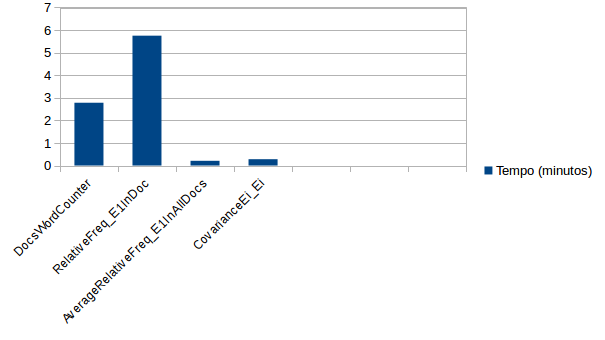
\includegraphics[height=3in]{LaTeX/Chapters/Figures/temposExecucao_Menores.png}
  \caption{Classes com os menores tempo de execução}
  \label{fig:temposExecucao_Menores}
\end{figure}

A classe \textit{ERFile\_Counter} registou um tempo de execução de aproximadamente 2 dias e meio, pois para cada documento é necessário calcular a frequência de cada ER. Ora num \textit{corpus} onde foram extraídas perto de 1 milhão de ERs, seria de esperar que tivessemos tempos de execução muito alargados. 14 segundos foi o tempo estimado para calcular uma covariância entre duas ERs, na classe \textit{CovarianceE1\_E2}. Para que esta pudesse produzir resultados em tempo útil, seria necessário que houvesse uma implementação paralela e distribuída. Para a classe \textit{CorrelationE1\_E2} extimou-se que o cálculo de uma correlação entre duas ERs demorasse cerca de 27 segundos; também neste caso, tornou-se necessária uma implementação paralela e distribuída. É de notar que, os tempos referidos de 14 e 27 segundos resultam de um programa ainda não otimizado. 

\section{Abordagem Paralela}
Para resolver a problemática da correlação estatística, assumindo sempre \textit{datasets} (corpus linguísticos) de grandes dimensões, elaborámos uma solução baseada em duas das frameworks de processamento paralelo mais usadas e também bem documentadas. Spark e Hadoop.

A meta que estas duas implementações pretendem atingir consiste em resolver com eficiência um dos problemas criados pelo crescimento do volume de dados. No âmbito deste problema, esta resolução assenta no cálculo da correlação entre grandes quantidades de pares de expressões relevantes. Este cálculo irá permitir que se criem ligações semânticas entre documentos e a construção automática de descritores de documentos. 

\subsection{Protótipo Hadoop MapReduce}
A solução produzida focou-se na implementação de um programa em MapReduce, preocupando-nos apenas em como processar corpora linguísticos de grandes dimensões de maneira eficiente. 

(ACHO QUE ESTE PARAGRAFO PODIA SAIR DAQUI, NAO FAZ MUITO SENTIDO) -> São várias as linguagens que podem ser utilizadas para produzir uma solução no paradigma MapReduce, suportadas pelo Hadoop. A discussão é muito entre qual linguagem a usar para produzir uma solução MapReduce. Python ou Java tendo em conta o contexto deste problema seriam as mais indicadas, no entanto com o aparecimento o Java 8 já existe mais apoio no que toca a programação funcional em funções lambda. Adjuvante a este facto, esta linguagem oferece uma quantidade considerável de bibliotecas úteis para ler documentos de texto e extrair/comprimir documentos no decorrer da execução do programa.

SECALHAR AQUI AINDA DEVIA DE FALAR DAS ESCRITAS QUE O MAPREDUCE FAZ PARA FICHEIRO E DE ALGUMA MANEIRA RELACCIONAR ISSO COM A QUANTIDADE DE DADOS PROCESSADO. EXPLICAR VANTAGENS E DESVANTAGENS.

Para calcular a correlação estatística, esta implementação divide-se em dois trabalhos MapReduce:
\begin{itemize}
    \item \textbf{1º trabalho consiste em: }contar as ocorrências de todas as ER's em cada documento; Calcular a frequência relativa de cada ER no respetivo documento; calcular a frequência relativa média para cada ER no corpus; valores intermédios tanto ao calculo da Covariância(ER1,ER2) como para a Covariância(ER1,ER1). 
    \item \textbf{2º trabalho: }Lê o output produzido pela 1ª tarefa, calcula valores intermédios do calcúlo da Cov(A,B) e Cov(A,A), calcula os valores finais para as duas covariâncias. E por fim calcula o resultado da correlação entre duas expressões relevantes. 
\end{itemize}

\subsubsection{Descrição Detalhada - 1º Trabalho MapReduce}
\subsubsubsection{Fase de Map}
Numa instância de Map existem mais duas funções para além da principal map(). Estas ocorrem sempre numa ordem específica: setup() -> map() -> cleanup(); O setup() é chamado apenas uma vez antes do inicio da tarefa; o cleanup() é chamado uma vez antes do final da tarefa. Tipicamente estas duas funções são usadas para carregar dados para a Cache das tarefa Map/Reduce, ou fazer uma ligação a uma base de dados, entre outras funções. Já o cleanup() é usado para o "inverso" da função setup(), fechar conexões a bases de dados, fechar escritas de ficheiros, entre outros.
Tendo como base o que foi descrito acima, utilizou-se o setup() para que cada tarefa de Map vá ter carregado para Cache um ficheiro que contém todas as expressões relevantes a correlacionar no corpus (RelevantExpressions.txt).

Depois do setup() a função que se segue é o map(). Tipicamente o input \textit{default} desta função está no formato \textit{TextInputFormat (Key, Value)}, em que a \textit{Key} corresponde ao \textit{offset} do inicío de cada linha e o \textit{Value} ao conteúdo da linha em si. Este trata cada linha de cada ficheiro de input forma separada. Ou seja, este tipo de formato é útil para dados desformatados ou ficheiros de \textit{log}. Primeiramente começou-se por usar este formato, mas rapidamente concluímos que seria melhor construir um formato próprio para o contexto do nosso problema. Para isso criou-se o \textit{WholeFileInputFormat (Key, Value)}, em que a Key corresponde ao nome do documento a processar e o Value ao texto em si.
Este formato permite que cada ficheiro que é dado como input não seja dividido em várias linhas pelas várias tarefas de mapper. Assim sendo cada tarefa Map irá processar unicamente um ficheiro por completo. Ou seja, irão ser criados o número de instâncias/tarefas de mappers igual ao número total de ficheiros. O processamento é feito desta maneira, pois o objetivo é extrair o máximo de informação de todos os documentos e expressões relevantes, processando-os uma só vez.

Depois da função map() receber o devido input: começa por contar as ocorrências de todas as ER's no documento; calcula a frequência relativa de todas as ER's que foram mapeadas nesse documento e por fim calcula resultados intermédios para o calculo da frequência relativa média das ER's, para a Cov(ER1, ER2), e Cov(ER1, ER1). O map() emite dois tipos de par (K,V) intermédios: ("SUM\_ER1,ER1", DoubleWritable) e ("MULTI\_ER1,ER2", DoubleWritable). Após estas chaves estarem escritas para disco, segue-se a fase do reduce.

\subsubsection{Fase de Reduce}
Tal como na fase de Mapping, numa tarefa de reduce, também existem as funções setup(), cleanup(), e são executadas exatamente nas mesmas condições. Tendo isto em conta, nesta tarefa a função setup() é utilizada para abrir a escrita de dois ficheiro do tipo \textit{SequenceFile}. Num deles irá ser escrito o resultado final da frequência relativa média de todas as ER's mapeadas pela fase de Mapping; O outro vai servir para escrever os resultados finais da covariância entre a mesma ER (Cov(ER1, ER1)).

Neste trabalho MapReduce só irá existir uma tarefa Reduce. É necessário que assim o seja, devido à natureza da formula da correlação de Pearson. Assim sendo, o reduce vai receber todos os pares (K,V) intermédios produzidos pelas tarefas de mapping.
Quando a função reduce() recebe uma chave do tipo "SUM\_ER1,ER1": calcula o resultado final tanto da frequência relativa média, como a Cov(ER1,ER1), e escreve-os para os \textit{SequenceFile's} respectivos. Ao receber uma chave do tipo "MULTI\_ER1,ER2" a função reduce() irá simplesmente agregar todos os valores correspondentes à respetiva chave e escrever para disco na respetiva forma, ("SUM\_COV(ER1,ER2)" , 0,0062). O formato do output escrito pelo reduce() é o \textit{default}, \textit{TextOutputFormat}. Este escreve um par \textit{(key, value)} em cada linha para um ficheiro de texto, em que a chave é escrita separada pela expressão regular "Tab" do valor. 
Por fim a função cleanup() irá apenas fechar a escrita dos dois \textit{SequenceFile's}.

\subsection{Descrição Detalhada - 2º Trabalho MapReduce}
\subsubsection{Fase de Map}
Nesta fase de Map, inicialmente na função setup() irá ser carregado para memória o \textit{SequenceFile} correspondente à frequência relativa média de cada expressão relevante. 

Como o output da função reduce() do 1º trabalho é do tipo \textit{TextOutputFormat}, consequentemente o input da função map() deste trabalho é \textit{KeyValueTextInputFormat}. Este formato é similar ao \textit{TextInputFormat}, também trata de cada linha do ficheiro de forma separada. No entanto o \textit{KeyValueTextInputFormat}(K,V) difere num aspeto. Este, vai partir a linha dada como input pela expressão regular "Tab". E à primeira parte corresponde a chave, e ao restante corresponde o valor. Exemplo: (SUM\_COV(ER1,ER2)    0,0062).

Posto isto, a função map() calcula a covariância entre duas ER's distintas, para cada par \textit{(Key,Value)} que recebe como input. Este calculo é realizado com o auxilio de valores extraídos do ficheiro que está em cache. Após o calculo da covariância concluir é emitida um par (K,V) intermédio, ("COV\_ER1\_ER2", DoubleWritable).

\subsubsection{Fase de Reduce}
O primeiro método a ocorrer nesta fase é o setup(), nele é carregado para memória o \textit{SequenceFile} correspondente à covariância entre a mesma expressão relevante, Cov(ER1,ER1). A função reduce() a cada chave que recebe vai agregar os seus valores, e calcular o resultado final da formula da correlação de Pearson entre duas expressões relevantes. Escreve então estes resultados para disco com o formato \textit{TextOutputFormat}.

FALTA INSERIR IMAGEM DO ESQUEMA DA SOLUÇÃO


\section{Protótipo Spark}
A solução desenhada para Spark, produzida em Scala, privilegia a utilização de RAM como modo de acelerar o processamento, ao revés de emitir escritas intermédias para disco como modo de precaver tolerância a falhas (\textit{fault tolerance}). Para tal utiliza o modelo de dados Resiliant Distributed Datasets(rdd's).

O RDD não executa as transformações que lhe são dadas, até ao momento em que recebe uma ação, tendo a característica de execução retardada (\textit{Lazy Evaluation}). Todas as dependências associadas ao RDD vão ser guardadas num grafo acíclico direcionado, independentemente dos dados. A isto chamamos um grafo de linhagem de Spark \cite{spark_transf}. Aquando a criação de um RDD novo a partir de um RDD existente, agrega-se a este um apontador para o RDD anterior, gerando assim um grafo acíclico direcionado. A cada transformação executada é gerada uma relação de dependencia com a transformação anterior, até ao caso base onde a transformação é o RDD pai.
A aplicação de transformaçoes gera uma cadeia de sucessão
Aquando cada transformaçao esta aponta para anterior para um grafo aciclico direccionado
A isto chama-se um grafo de linhagem. Linhagem de um RDD é no fundo um grafo com todas as dependências dos RDDs pais para ele\ref{RDD_DAG}.



\begin{figure}[htbp]
\label{RDD_DAG}
	\centering
	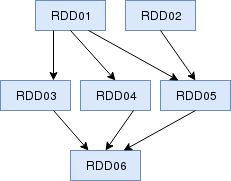
\includegraphics[height=1.8in]{LaTeX/Chapters/Figures/RDD_DAG.png}
  \caption{Grafo de linhagem dos RDDs}
  \label{fig:fluxo_execucao}
\end{figure}


Avoiding disk I/O, contributes to a faster solution, since RAM access is several orders of mignitude faster that disk. RAM is more expensive than lower access storage altenatives, and as such it becomes a scarce resource. Thus, storing the full dataset in-memory, yeilds a critial space constraint. Even more, when solving problems based on conbinations, where the original data itself generates exponential amount of new information, to be further processed.

% O Spark ao privilegiar o uso da RAM como modo de processamento, pode demonstrar também algumas desvantagens. A execução \textit{in-memory} pode ser um dos casos de \textit{bottleneck} quando desejamos processar eficientemente grandes quantidades de dados. Como o problema visa resolver uma grande quantidade de combinatória de ER's mapeadas pelo corpus, o uso de memória pode vir a demonstrar-se muito alto. Manter dados em memória é caro, o Apache Spark requer muita RAM para processar em memória. Logo os custos do Spark podem vir a revelar-se altos. % 

Tal como referido na secção \ref{estadoARte_spark}, há 2 tipos de operações que se podem aplicar num RDD. Vamos apenas dar ênfase nos métodos utilizados para esta solução e compara-los. 


Existem quatro variantes que traduzem a operação de mapping sobe um dado RDD, recebendo como parametro uma função que rege a transformação, e executando iterativamente sobre cada elemento:
\begin{description}
    \item [Map] é aplicado ao escopo do RDD, produzindo apenas um resultado.
    \item [FlatMap] similar ao Map, mas pode produzir múltiplos resultados
    \item [MapPartition] é aplicado a cada partição de um RDD, produzindo uma sequencia de resultados por partição.
    \item [MapPartitionsWithIndex] Proporciona o mesmo que o MapPartition, mas inclui juntamente com o resultado de cada partição, o seu respetivo índice no RDD. 
\end{description}
%Dentro das transformações \cite{spark_transf} há suporte para métodos do tipo \textit{map(func)}, que percorre cada elemento do RDD anterior aplicando-lhe uma função \textit{func}. Por outro lado o \textit{mapPartitions(func)} processa cada partição (bloco) do RDD em separado aplicando uma função \textit{func}.
%

Para o processamento de grandes quantidades de dados, o método de mapping MapPartitons é o mais adequado,pois.....

grandes quantidades de dados o método \textit{mapPartitions} consegue obter melhor performance em relação ao \textit{map}, por conseguir processar cada bloco do RDD em separado. 


São suportadas ainda transformações de agregação, \textit{reduceByKey(func)} foi o método utilizado para agregar os nossos dados nesta solução. Quando é chamado num \textit{RDD(Key, Value)}, retorna outro \textit{RDD(K,V)} onde os valores de cada chave são agregados segundo uma função \textit{reduce func}. O \textit{groupByKey()} por outro lado também consegue produzir exatamente o mesmo resultado, no entanto não oferece tão boa performance. A razão pela qual isto acontece deve-se ao facto do \textit{reduceByKey} combinar os valores de cada chave para cada partição antes de enviar os dados para a rede, isto faz com que na fase de \textit{shuffle} sejam enviados menos dados. \textit{Shuffle} consiste numa operação de muitos-para-muitos (NxN), em que vai ler a informação de todas as partições e encontrar todos os valores correspondentes a cada chave, agregando-os. Já o \textit{groupByKey} manda todos os pares (K,V), para a fase de \textit{shuffle}, sem os combinar primeiro dentro de cada partição (bloco) de dados, isto faz com que haja muita informação a ser enviada para a rede sem qualquer necessidade.

As ações \cite{spark_action} utilizadas neste protótipo foram:
\begin{itemize}
    \item \textit{collect()}- retorna todos os elementos de um RDD para um vetor alocado no \textit{driver program};
    \item \textit{collectAsMap()}- retorna todos os elementos de um RDD para um mapa alocado no \textit{driver program};
    \item \textit{count()} - conta o número total de elementos de um RDD para uma variavél no \textit{driver program};
    \item \textit{saveAsTextFile(path)} - escreve todos os elementos pertencentes a um RDD para um ficheiro de texto, dada uma diretoria (sistema de ficheiros local, HDFS, entre outros).
\end{itemize}

\subsection{Descrição detalhada - Protótipo Spark}
Analogamente ao protótipo MapReduce, esta solução visa processar eficiente corpora linguísticos de grandes dimensões. Com o objetivo de calcular a correlação estatística entre duas expressões relevantes, a implementação faz uso de vários RDD's interligados entre si. A versão do Spark utilizado foi a 2.3.0, recorrendo a Scala, na versão 2.11.8. 

O Spark consegue criar dados de forma distribuída a partir de qualquer tipo sistema armazenamento de dados  suportado pela Apache Hadoop, incluindo o sistema de ficheiros local, HDFS, Cassandra, Amazon S3, entre outros. Como input o Spark suporta \textit{SequenceFiles}, ficheiros de texto, ou outro \textit{InputFormat} do Hadoop. 

Tendo isso em conta, foram usados dois métodos diferente para conseguir carregar todos os dados necessários para fazer os cálculos da correlação. O \textit{SparkContext.textFile(path/to/directoryOrFile)} que cria um RDD a partir de um input do tipo \textit{URI}, como por exemplo: file:///, hdfs://, s3a://. Ao criar um RDD com este método ele irá retornar uma linha de cada vez por cada ficheiro, a framework irá criar uma partição por cada bloco do ficheiro. No HDFS os blocos têm de tamanho \textit{default} 128MB, que foi o sistema de armazenamento de dados utilizado para suportar este protótipo de Spark.  A outra função usada foi \textit{SparkContext.wholeTextFiles(path/to/directoryOrFile)}, esta lê uma diretoria com múltiplos ficheiros. Ao contrário do \textit{textFile()} este retorna um par (nome do ficheiro, texto) para cada ficheiro.

Existem dois RDD's que são responsáveis por guardar toda a informação do corpus a processar. O (relevantExpressionsRDD) foi construído pelo uso do \textit{textFile}, e contém todas as expressões relevantes a correlacionar. E o (allFilesRDD) que usou o \textit{wholeTextFiles}, guardando todos os documentos de texto pertencentes ao corpus linguístico.

De seguida há 2 RDDs diretamente dependentes do allFiles\_RDD, que fazem uso do \textit{mapPartitions}. Um deles, CounterAllWordsDoc\_RDD, está encarregado de contar o total de palavras em cada ficheiro de texto pertence ao corpus. Já o ERCounter\_RDD, conta o número de ocorrências de todas as expressões relevantes encontradas para cada ficheiro de texto. Para que o mapeamento das ER's seja realizado, chamamos a função \textit{collect()} no relevantExpression\_RDD e fornecemos como input ao ERCounter\_RDD, assim este RDD fica a depender de dois.

A fase que se segue, é o calculo da frequência relativa para cada expressão relevante encontrada em cada documento de texto. Para isso, recorrendo ao método \textit{mapPartitions}, são criados dois RDD's que possuem as mesmas dependências. Sendo elas: ERCounter\_RDD e CounterAllWordsDoc\_RDD. O MultiRelFreq\_RDD está incumbido de calcular valores intermédios para a covariância entre duas ER's diferentes. Após esse calculo é-lhe aplicada um método de agregação, \textit{reduceByKey(func)}. SumRelFreq\_RDD é responsável por calcular valores intermédios para a obtenção das frequências relativas médias de todas as ER's, aplicando-lhe também a transformação \textit{reduceByKey(func)}. Apesar destes dois RDD's calcularem a frequência relativa das mesmas ER's, eles tratam dos dados de maneira diferente, pois cada um deles produz valores intermédios para uma formula diferente. Um para a covariância e outro para a frequência relativa média. A outra hipótese que teríamos para efetuar estes cálculos, passaria pela criação de um RDD dotado para produzir os resultados intermédios que o MultiRelFreq\_RDD, e o SumRelFreq\_RDD. Posteriormente a isso iria ter de ser aplicada uma transformação do tipo \textit{filter(func)}, filtrando assim e separando as chaves para dois RDDs separados. Como o problema a resolver trata de uma grande quantidade de dados, não seria viável estar a "varrer" duas vezes de seguida o mesmo RDD para o separar em dois. Isto iria oferecer uma complexidade temporal ao protótipo desnecessária.

Para finalizar o calculo da frequência relativa média é gerado um RDD (AVGRelFreq\_RDD) que utiliza o \textit{mapPartitions}. Este RDD depende de SumRelFreq\_RDD.

Para o calculo da covariância entre a mesma expressão relevante, foi criado o SumPowRelFreq\_RDD que depende diretamente de SumRelFreq\_RDD. Mas também o CovAA\_RDD que depende de SumPowRelFreq\_RDD e de AVGRelFreq\_RDD. O SumPowRelFreq\_RDD mapeia todos valores para o seu quadrado, e aplica o \textit{reduceByKey(func)}. O CovAA\_RDD faz uso do \textit{mapPartitions}, calculando assim o resultado final para a covariância entre a mesma ER.

Por fim o último RDD a ser formulado foi o CorrelationAB\_RDD. Este depende de CovAA\_RDD; AVGRelFreq\_RDD; e MultiRelFreq\_RDD. Aplicando também o \textit{mapPartitions}, este calcula o valor final da covariância entre duas ER's diferentes, e posteriormente a isso produz o output final, sendo ele a correlação estatística de Pearson.

FALTA INSERIR IMAGEM DO ESQUEMA DA SOLUÇÃO
 